% ----------------------------------------------------------
% PARTE
% ----------------------------------------------------------
\part{Referenciais teóricos}
% ----------------------------------------------------------

% ---
% Capitulo de revisão de literatura
% ---
\chapter{Big Data}
% ---

Não existe uma definição clara do que é Big Data. Inicialmente, trata-se de um volume de informações que cresceu de tal forma que simples computadores não são capazes de processar com ferramentas tradicionais\cite[p. 6]{CUKIER}. Big Data pode se referir a qualquer ação ou evento que necessite ser executado em larga escala e não é possível ser realizado numa estrutura menor, para extrair novos insights ou criar novas formas de valor de tal forma que provoque mudanças nos mercados, organizações, na relação entre as pessoas e os governos, entre outros.


Big data é a habilidade da sociedade em aproveitar informações de novas maneiras para produzir insights or bens e serviços com um valor significativo\cite[p. 2]{CUKIER}. Para o autor, os dados não ficam mais num estado estático, isto é, quando depois de sua coleta, não existe uma serventia se não o seu simples armazenamento. Caso sejam utilzados da forma correta, os dados podem ser reutilizados, tornando-se uma fonte de inovação e novos serviços.

Para \cite[p. 5]{ZIKO}, Big Data pode ser caracterizado por:

\begin{itemize}
  \item Volume: refere-se a grande volume de dados gerados. Dentre os desafios, em grande parte resolvidos, estão que tipo de tecnologia a ser utilizada para guardar um volume grande de dados, uma vez que as tradicionais são incapazes ou ineficientes para lidar com essa questão, além do custos de armazenagem.
  \item Velocidade: relacionado a rapidez com que os dados são gerados. Com a evolução da tecnologia, tudo está cada vez mais interconectado. As bandas largas possibilitam um tráfegos de dados cada vez maior e mais eficiente. Sistemas de tempo real passaram a ter maior relevância para as empresas, que podem tomar decisões cada vez mais rápida.
  \item Variedade: trata-se dos diferentes dispositivos que podem gerar dados passíveis de extração de informação. Smartphones, tables, internet das coisas, computadores, sensores podem produzir dados em diferentes formatos que precisam ser interpretados e armazenados.
  \item Valor: é o aspecto mais subjetivo e complexo, porém estratégico. Representa o que o Big Data pode gerar de informação a partir de dados brutos.
\end{itemize}











\subsection{Segmentação}


Com um volume de dados grande disponível, uma possibilidade para as empresas é conseguir reconhecer certos padrões. Por exemplo, conhecendo o perfil dos clientes, é possível adotar estratégias adequadas para cada segmento, principalmente quando o público alvo é composto por clientes muito heterogêneos. Segundo \citeonline[p. 257]{KOTLER}, ``segmentação de mercado é o ato de dividir um mercado em grupos distintos de compradores com diferentes necessidades e respostas''.

\begin{citacao} 
Um bom agrupamento exibe a característica de que objetos associados ao mesmo grupo são bastante similares, ao mesmo tempo em que objetos associados a grupos diferentes exibem uma baixa similaridade. Aplicações diretas da análise de grupos incluem segmentação de clientes ou de produtos, agrupamento de genes em um experimento de micro-array, organização dos resultados de uma consulta enviada a um mecanismo de busca da WEB, etc.
\cite{BEZERRA} \end{citacao}

Com a segmentação e os grupos definidos, é possível realizar uma análise descritiva para traçar um padrão no comportamento dos dados. 

% ---
\subsubsection{K Médias}
% ---

O K Médias é um algoritmo de \emph{machine learning} não supervisionado relativamente simples, podendo ser utilizado para resolver problemas de clusterização. Para \citeonline{MacQueen}, trata-se de um método que tem para uma quantidade k de \emph{clusters} pré definida, o objetivo de definir k centróides\footnotemark \footnotetext{centróide é um conceito muito utilizado em geometria e física e representa um ponto médio ou um centro de massa de uma representação. No caso de K Médias, considerando que as informações são transformadas em vetores, seria um ponto médio da informação}, um para cada \emph{cluster}, tal que o conjunto de dados possa ser repartido de forma eficiente. Para um conjunto de observações \begin{math}(x_{1}, x_{2}, ..., x_{n})\end{math}, onde 

\begin{equation}
\label{eq:media}
\underset{S}{\arg\min} \sum_{i=1}^{k} \sum_{x \in S_{i}}\left \| x - \mu_{i} \right \|^{2},
\end{equation}

onde \begin{math}\mu_{i}\end{math} é a média dos pontos em \begin{math}S_{i}\end{math}

O algoritmo minimiza a função objetiva usando o princípio dos mínimos quadrados. Por conta disso, é sensível a \emph{ouliers} e ruídos. O pseudo algoritmo do K Médias seria estes passos:\\

\begin{algorithm}[H]
\SetAlgoLined
 1. Defina uma inicialização inicial aleatória usando k \emph{clusters}\;
 \While{Não houve convergência}{
   2. Atribua para cada ponto do conjunto de dados um \emph{cluster} mais próximo\;
   3. Redefina a posição do centróide de cada \emph{cluster} como um ponto médio de todos os pontos do \emph{cluster}\;
 }
 \caption{K Médias}
\end{algorithm}

\vspace{5mm}


\begin{figure}[!ht]
\caption{Evolução da execução do algoritmo de K Médias }
\centerline{\includegraphics[width=0.5\textwidth]{img/k-means}}
\fonte{Extraído de \cite{kmeans-step}}
\end{figure}



A localização desses centróides deve ser o mais afastado entre si possível. A partir de uma posição inicial dos centróides, o próximo passo é, então, associar todos pontos do conjunto de dados com o centróide mais próximo. Com os pontos associados, recalcula-se k novos centróides como baricentros dos \emph{clusters} anteriores, repetindo esses passos até que os novos centróides sejam gerados muito próximos do passo anterior. 





% ---
\section{Classificação}
% ---

A classificação é uma análise preditiva com o objetivo de estabelecer modelos que possbilitem uma previsão do futuro, permitindo estudar tendências por meio do uso de técnicas estatísticas sobre dados históricos.

\subsection{Regressão Linear}


A regressão linear é uma modelagem matemática \footnotemark \footnotetext{modelagem matemática é uma representação em fórmulas matemáticas que tentam descrever ou simular eventos e sistemas reais com o propósito de prever comportamentos} que permite descrever variáveis em função de outras. Segundo \citeonline[p. 44]{HASTIE} ela pode ser representada como
\begin{equation}
  \label{eq:regressao_linear}
  \begin{aligned}
Y &= \hat{\beta_{0}} + \sum_{j=1}^{p} (X_{j}\hat{\beta_{j}}), 
  \end{aligned}  
\end{equation}
onde \begin{math}Y\end{math} representa uma variável dependente contínua, \begin{math}X_{j}\end{math} as variáveis independentes (contínuas, discretas ou binárias). Isto significa que uma certa característica (variável dependente) pode ser descrita por outras (variável independente).

Para ajustar o modelo linear ao conjunto de dados, é possível utilizar diferentes maneiras. Um deles é método dos mínimos quadrados, uma técnica de otimização matemática que visa encontrar ajuste ótimo para um conjunto de dados por meio da minimização a soma dos quadrados das diferenças entre o valor estimado e os dados observados, representado por:

\begin{equation}
  \label{eq:minimos_quadrados}
  \begin{aligned}
G(\beta) &= \sum_{i=1}^{N} (y_{i}-x_{i}^{T}\beta)^{2}, 
  \end{aligned}  
\end{equation}

Assim, nosso problema passar a ser como descobrir \begin{math}\hat{\beta}\end{math} que minimize \ref{eq:minimos_quadrados}. Para calcular \begin{math}\hat{\beta}\end{math}, é possível utilizar a equação:

\begin{equation}
  \label{eq:solucao_minimos_quadrados}
  \begin{aligned}
\hat{\beta} &= (X^{T}X)^{-1}X^{T}y, 
  \end{aligned}  
\end{equation}

onde \begin{math} X \in \mathbb{R}^{N,p} \end{math} X representando uma matriz com cada linha sendo um vetor do conjunto de dados de entrada e \begin{math}y \in \mathbb{R}^{N}\end{math} um vetor que representa os dados de saída \footnotemark \footnotetext{inicialmente, esses dados devem vir do conjunto de treino}

Com a definição de \begin{math}\hat{\beta}\end{math}, é possível determinar uma reta que separa o conjunto de dados.

\begin{figure}[!ht]
\caption{Exemplo de classificação em 2 dimensões.}
\centerline{\includegraphics[width=0.5\textwidth]{img/hiperplano}}
\fonte{Extraído de \cite{HASTIE}}
\end{figure}

 As classes estão representadas um variável binária (AZUL = 0, LARANJA = 1), ajustadas por uma regressão linear. A linha que separa os grupos foi definido por \begin{math}x^{T}\hat{\beta} = 0,5\end{math}. A área hachurada em laranja representa o espaço classificado por LARANJA enquanto a área em azul, classificado por AZUL

\subsection{Regressão Logística}

Segundo \citeonline[p. 119]{HASTIE}, a regressão logística, assim como a regressão linear, também é um modelo matemático de predição de eventos usada para descrever dados e explicar a relação entre um conjunto de variáveis independentes e uma variável dependente. Contudo, enquanto na regressão linear a variável dependente é contínua, na regressão logística, ela é considerada uma variável categórica. Ela segue uma distribuição Bernoulli\footnotemark \footnotetext{distribuição de Bernoulli é uma modelagem de probabilidade que representa eventos binários cujas ocorrências são tratados como sucesso ou falha. Considerando que a probabilidade de ocorrer um sucesso é \begin{math}p\end{math}, então a probabilidade de ocorrer uma falha é \begin{math}1-p\end{math} } com uma probabilidade \begin{math}p\end{math} desconhecida. Assim, a regressão logística tem como objetivo estimar essa probabilidade \begin{math}p\end{math} desconhecida.

Para estimar essa probabilidade, a regressão logística usa as chances (\emph{odds}) do evento ocorrer em cada variável independente, calculando a taxa dessas chances, dada pela equação:

\begin{equation}
  \label{eq:OR}
  \begin{aligned}
   OR &= \frac{P(sucesso)}{P(fracasso)}\\
     &= \frac{p}{1-p}
  \end{aligned}
\end{equation}

Utilizando inferência de estatística, podemos aplicar log em \ref{eq:OR}, ficando com:

\begin{equation}
  \label{eq:t}
  \begin{aligned}
    logit(p) &= ln\left ( \frac{p}{1-p} \right )
  \end{aligned}
\end{equation}

Tal transformação recebe o nome de logit. Ela é ajustada a função de predição, como numa análise de regressão linear, visto anteriormente. O valor final obtido a partir da função logit é convertido novamente para as chances via a função inversa do logaritmo natural (ou uma função exponencial).

\begin{equation}
  \label{eq:t}
  \begin{aligned}
    logit^{-1}(\alpha) &= \frac{1}{1+e^{-\alpha}} &= \frac{e^{\alpha}}{1+e^{\alpha}}
  \end{aligned}
\end{equation}

\begin{figure}[!ht]
\caption{Fun\c c\~ao logit}
\centerline{\includegraphics[width=.6\textwidth]{img/logit}}
\fonte{Gerado a partir do script}
\end{figure}


Generalizando, temos:

\begin{equation}
  \label{eq:t}
  \begin{aligned}
    \log\left ( \frac{P(G = 1 | X = x)}{P(G = K | X = x)} \right ) &= \beta_{10}+\beta_{1}^{T}x\\
    \log\left ( \frac{P(G = 2 | X = x)}{P(G = K | X = x)} \right ) &= \beta_{20}+\beta_{2}^{T}x\\
    \log\left ( \frac{P(G = K-1 | X = x)}{P(G = K | X = x)} \right ) &= \beta_{(k-1)0}+\beta_{k-1}^{T}x,
  \end{aligned}
\end{equation}

onde o modelo é composto por K classes e K - 1 transformações logit. Utilizando a inversa da logit, temos:

\begin{equation}
  \label{eq:t}
  \begin{aligned}
    P(G = k | X = x) &= \frac{\exp \left ( \beta_{k0}+\beta_{k}^{T}x \right )}{1 + \sum_{\ell=1}^{K - 1}\exp \left ( \beta_{\ell0}+\beta_{\ell}^{T}x \right )}, k = 1, ..., K - 1\\
    P(G = K | X = x) &= \frac{1}{1 + \sum_{\ell=1}^{K - 1}\exp \left ( \beta_{\ell0}+\beta_{\ell}^{T}x \right )}
  \end{aligned}
\end{equation}

Dessa forma, temos que a regressão logística estima as changes (odds) como uma variável contínua, mesmo quando a variável dependente que está sendo o objeto de estudo seja uma variável binária. 



\begin{comment} 
\begin{citacao} 
\cite{HASTIE} \end{citacao}
, mas que leva em consideração as probabilidades de ocorrência desses eventos.
\end{comment}

Assim, a regressão logística viabiliza a classificação das observações por meio da probabilidade estimada na categoria estudada.


% ---
\section{\emph{Random Forest}}


\subsection{Árvores}

% ---
Árvores são modelos presentes tanto em computação como estrutura de dados e em estatística como estrutura para tomadas de decisão. No contexto de \emph{Machine Learning}, a árvore de decisão refere-se a uma estrutura de modelo preditivo, um método de aprendizagem supervisionada não parametrizada utilizada para classificação (para variáveis categóricas) e regressão (variáveis métricas). Trata-se de um modelo de conjunto de decisões ou regras na qual estabelece um fluxo dentro de sua estrutura, definindo uma classificação ou uma predição. Para \citeonline[p. 305]{HASTIE}, as árvores permitem um particionamento do espaço em um conjunto regiões. Suponha que exista \begin{math}M\end{math} partição que possa ser divida em regiões \begin{math}R_{1}, R_{2}, ..., R_{M} \end{math} e que seja possível modelar a resposta para cada região com a constante \begin{math}c_{m}\end{math}, 

\begin{equation}
f(x) = \sum_{m=1}^{M}c_{m}I( x \in R_{m} )
\end{equation}

Para a repartição dessas regiões, são definidos critérios para decidir de qual lado o dado irá ficar na árvore. São estruturas de fácil interpretação pois, uma vez criado o modelo, percorrer os nós da árvore indica as características do dado.


\tikzset{
  treenode/.style = {shape=rectangle, rounded corners,
                     draw, align=center,
                     top color=white, bottom color=blue!20},
  root/.style     = {treenode, font=\Large, bottom color=purple!30},
  env/.style      = {treenode, font=\ttfamily\normalsize},
  dummy/.style    = {circle,draw}
}

\begin{figure}[!ht]
\caption{Exemplo de árvore classificadora}
\centering
        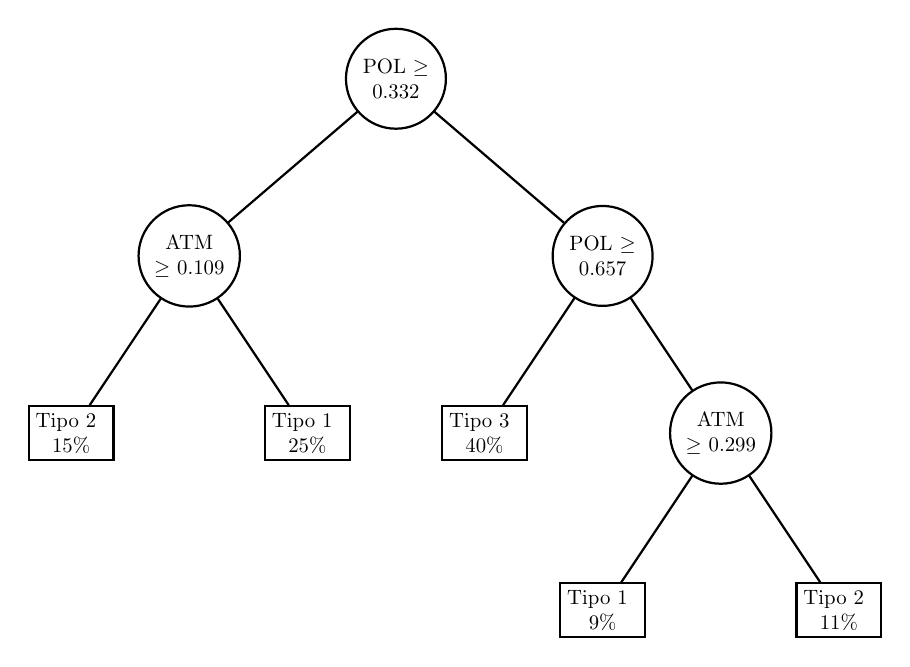
\begin{tikzpicture}[thick,scale=0.75, every node/.style={scale=0.75}]
\node [circle,draw,text width=1.2cm,align=center]{POL $\ge$ 0.332} [level distance=30mm,sibling distance=70mm]
child {node [circle,draw,text width=1.2cm,align=center] {ATM $\ge$ 0.109 } [level distance=30mm ,sibling distance=40mm]
child {node [rectangle,draw,text width=1.2cm,align=center] {Tipo 2\newline15\%}}
child {node [rectangle,draw,text width=1.2cm,align=center] {Tipo 1\newline25\%}}
}
child { node [circle,draw,text width=1.2cm,align=center]{ POL $\ge$ 0.657} [level distance=30mm ,sibling distance=40mm]
child {node [rectangle,draw,text width=1.2cm,align=center] {Tipo 3\newline40\%}}
child { node [circle,draw,text width=1.2cm,align=center]{ ATM $\ge$ 0.299 } [level distance=30mm ,sibling distance=40mm]
child {node [rectangle,draw,text width=1.2cm,align=center] {Tipo 1\newline9\%}}
child {node [rectangle,draw,text width=1.2cm,align=center] {Tipo 2\newline11\%}}
}
};
\end{tikzpicture}
\nota{Cada nó representa um atributo de um elemento da amostra. As folhas são consideradas a representação da classe a que uma observação pertence. Já o ramo é um conjunto de valores que reflete todas suas características e detalhes de um elemento}
\fonte{Criado pelo autor}
\end{figure}

\subsubsection{Árvore de regressão}

Para \citeonline[p. 307]{HASTIE}, árvores de regressão são utilizadas em problemas de predição. Assim, a variável de saída refere-se a uma variável numérica e contínua.

Assim como foi visto anteriormente, o algoritmo deve conseseguir decidir em quais variáveis e quais pontos as decisões serão tomadas, construindo a topologia da árvore.

No caso de uma regressão, poderia utiliza-se como critério de minimização a soma do mínimos quadrados \begin{math}\sum{ (y_{i} - f(x_{i}))^{2}}\end{math}, temos que o melhor \begin{math}\hat c_{m}\end{math} é exatamente a média para \begin{math}y_{i}\end{math} na região \begin{math}R_{m}\end{math}:

\begin{equation}
\label{eq:media}
\hat c_{m} = m\acute edia(y_{i} | x_{i} \in R_{m})
\end{equation}

Para encontrar a melhor partição, é necessário recorrer a um algoritmo guloso\footnotemark \footnotetext{\emph{algoritmo guloso} é um algoritmo que  busca a resolução de um problema elegendo sempre uma solução localmente ótima. Isto significa que, dentro de um conjunto de soluções possíveis numa determinada etapa da solução do problema, escolhe-se sempre a que traz o melhor resultado naquela situação, o que muitas vezes pode não levar a uma solução ótima global.}, uma vez que calcular utilizando os mínimos quadrados é computacionalmente inviável.

Seja \begin{math}j\end{math} uma variável de reparticionamento, $s$ um ponto de divisão. É possível definir um par de semi planos 

\begin{equation}
R_{1}(j,s) = {X | X_{j}\leq s} \quad \textrm{e} \quad R_{2}(j,s) = {X | X_{j}\textgreater s})
\end{equation}

Resultando a busca pela de \begin{math}s\end{math} e \begin{math}j\end{math} que resolva

\begin{equation}
\min_{j,s} \left [ \min_{c_{1}} \sum_{x_{i} \in R_{1} (j,s)} (y_{i} - c_{1})^{2} + \min_{c_{1}} \sum_{x_{i} \in R_{2} (j,s)}(y_{i} - c_{2})^{2} \right ]
\end{equation} 


Mas como visto em \ref{eq:media}, temos que para qualquer $j$ e $s$, a minimização interna pode ser resolvida por:

\begin{equation}
\hat c_{1} = m\acute edia(y_{i} | x_{i} \in R_{1}(j,s)) \quad \textrm{e} \quad \hat c_{2} = m\acute edia(y_{i} | x_{i} \in R_{2}(j,s))
\end{equation} 

Este processo é repetido até que todas as regiões sejam descobertas.

\subsubsection{Árvore de classificação}

Para o caso de uma árvore de classificação, \citeonline[p. 308]{HASTIE} explica que o objetivo principal concentra-se em conseguir, a partir das variáveis independentes, efetuar a decisão em definir um classe para uma determinada entrada de dados. Logo, a saída é uma variável categórica.
Neste caso, utiliza-se como critério de decisão o índice de Gini\footnotemark \footnotetext{Índice de Gini mede a frequencia de que um elemento selecionado aleatoriamente de um conjunto é marcado de forma errada}
\begin{math}Gini(T) = 1 - \sum_{i=1}^{n}{ p_{i}^{2}}\end{math},
onde p é a proporção de observações de uma determinada classe para um dado nó.

\subsection{\emph{Bagging}}

As árvores vistas anteriormente são modelos interessantes de classificação mas possuem um problema: o resultado gerado por elas em geral possuem uma acurácia muito baixa quando a estrutura da árvore começa a crescer muito \cite[p. 312]{HASTIE}.
A proposta do \emph{Bagging} é criar subconjuntos dos dados, gerando diversas árvores que deverão executar a classificação. Esses modelos subconjuntos são gerados com reposição, ou seja, um mesmo dado pode estar presente em mais de um modelo no momento do treino. Cada árvore gerada fornecerá um modelo para a \emph{Random Forest} e um valor intermediário será adotado para os nós. 

\begin{figure*}[ht!]
    \centering
        \caption{Exemplo de composição da \emph{Random Forest}}
    \begin{subfigure}[t]{0.5\textwidth}
        \centering
        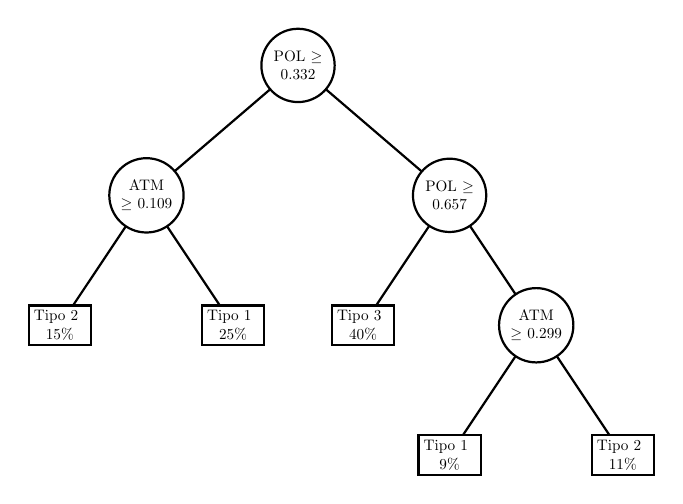
\begin{tikzpicture}[thick,scale=0.55, every node/.style={scale=0.55}]
\node [circle,draw,text width=1.2cm,align=center]{POL $\ge$ 0.332} [level distance=30mm,sibling distance=70mm]
child {node [circle,draw,text width=1.2cm,align=center] {ATM $\ge$ 0.109 } [level distance=30mm ,sibling distance=40mm]
child {node [rectangle,draw,text width=1.2cm,align=center] {Tipo 2\newline15\%}}
child {node [rectangle,draw,text width=1.2cm,align=center] {Tipo 1\newline25\%}}
}
child { node [circle,draw,text width=1.2cm,align=center]{ POL $\ge$ 0.657} [level distance=30mm ,sibling distance=40mm]
child {node [rectangle,draw,text width=1.2cm,align=center] {Tipo 3\newline40\%}}
child { node [circle,draw,text width=1.2cm,align=center]{ ATM $\ge$ 0.299 } [level distance=30mm ,sibling distance=40mm]
child {node [rectangle,draw,text width=1.2cm,align=center] {Tipo 1\newline9\%}}
child {node [rectangle,draw,text width=1.2cm,align=center] {Tipo 2\newline11\%}}
}
};
\end{tikzpicture}

        \caption{Configuração 1 da árvore de decisão}
    \end{subfigure}%
    ~ 
    \begin{subfigure}[t]{0.5\textwidth}
        \centering
        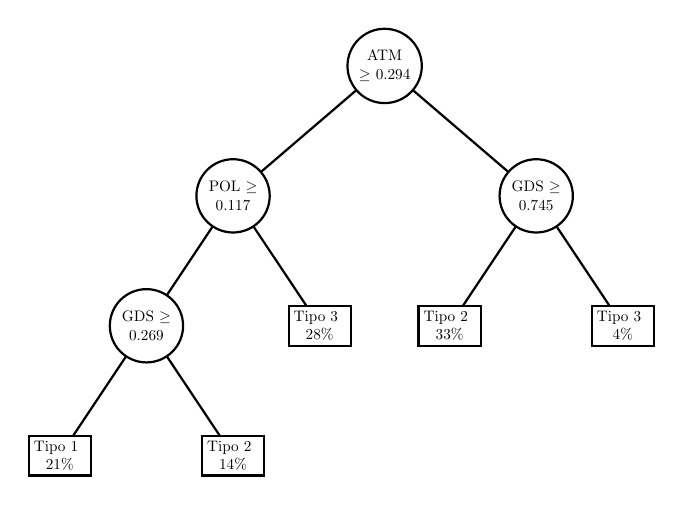
\begin{tikzpicture}[thick,scale=0.55, every node/.style={scale=0.55}]
\node [circle,draw,text width=1.2cm,align=center]{ATM $\ge$ 0.294} [level distance=30mm,sibling distance=70mm]
child { node [circle,draw,text width=1.2cm,align=center]{ POL $\ge$ 0.117 } [level distance=30mm ,sibling distance=40mm]
child { node [circle,draw,text width=1.2cm,align=center]{ GDS $\ge$ 0.269 } [level distance=30mm ,sibling distance=40mm]
child {node [rectangle,draw,text width=1.2cm,align=center] {Tipo 1\newline21\%}}
child {node [rectangle,draw,text width=1.2cm,align=center] {Tipo 2\newline14\%}}}
child {node [rectangle,draw,text width=1.2cm,align=center] {Tipo 3\newline28\%}}
}
child {node [circle,draw,text width=1.2cm,align=center] { GDS $\ge$ 0.745 } [level distance=30mm ,sibling distance=40mm]
child {node [rectangle,draw,text width=1.2cm,align=center] {Tipo 2\newline33\%}}
child {node [rectangle,draw,text width=1.2cm,align=center] {Tipo 3\newline4\%}}
};
\end{tikzpicture}
        \caption{Configuração 2 da árvore de decisão}
    \end{subfigure}
\fonte{Criado pelo autor}
\end{figure*}



% \begin{figure*}[t!]
%     \centering
%     \begin{subfigure}[t]{0.5\textwidth}
%         \centering
%         \begin{tikzpicture}[thick,scale=0.55, every node/.style={scale=0.55}]
% \node [circle,draw,text width=1.2cm,align=center]{POL $\ge$ 0.332} [level distance=30mm,sibling distance=70mm]
% child {node [circle,draw,text width=1.2cm,align=center] {ATM $\ge$ 0.109 } [level distance=30mm ,sibling distance=40mm]
% child {node [rectangle,draw,text width=1.2cm,align=center] {Tipo 2\newline15\%}}
% child {node [rectangle,draw,text width=1.2cm,align=center] {Tipo 1\newline25\%}}
% }
% child { node [circle,draw,text width=1.2cm,align=center]{ POL $\ge$ 0.657} [level distance=30mm ,sibling distance=40mm]
% child {node [rectangle,draw,text width=1.2cm,align=center] {Tipo 3\newline40\%}}
% child { node [circle,draw,text width=1.2cm,align=center]{ ATM $\ge$ 0.299 } [level distance=30mm ,sibling distance=40mm]
% child {node [rectangle,draw,text width=1.2cm,align=center] {Tipo 1\newline9\%}}
% child {node [rectangle,draw,text width=1.2cm,align=center] {Tipo 2\newline11\%}}
% }
% };
% \end{tikzpicture}

%         \caption{Configuração 1 da árvore de decisão}
%     \end{subfigure}%
%     ~ 
%     \begin{subfigure}[t]{0.5\textwidth}
%         \centering
%         \begin{tikzpicture}[thick,scale=0.55, every node/.style={scale=0.55}]
% \node [circle,draw,text width=1.2cm,align=center]{ATM $\ge$ 0.294} [level distance=30mm,sibling distance=70mm]
% child { node [circle,draw,text width=1.2cm,align=center]{ POL $\ge$ 0.117 } [level distance=30mm ,sibling distance=40mm]
% child { node [circle,draw,text width=1.2cm,align=center]{ GDS $\ge$ 0.269 } [level distance=30mm ,sibling distance=40mm]
% child {node [rectangle,draw,text width=1.2cm,align=center] {Tipo 1\newline21\%}}
% child {node [rectangle,draw,text width=1.2cm,align=center] {Tipo 2\newline14\%}}}
% child {node [rectangle,draw,text width=1.2cm,align=center] {Tipo 3\newline28\%}}
% }
% child {node [circle,draw,text width=1.2cm,align=center] { GDS $\ge$ 0.745 } [level distance=30mm ,sibling distance=40mm]
% child {node [rectangle,draw,text width=1.2cm,align=center] {Tipo 2\newline33\%}}
% child {node [rectangle,draw,text width=1.2cm,align=center] {Tipo 3\newline4\%}}
% };
% \end{tikzpicture}
%         \caption{Configuração 2 da árvore de decisão}
%     \end{subfigure}
%     \\
%     \centering
%     \begin{subfigure}[t]{0.5\textwidth}
%         \centering
%         \begin{tikzpicture}[thick,scale=0.55, every node/.style={scale=0.55}]
% \node [circle,draw,text width=1.2cm,align=center]{POL $\ge$ 0.332} [level distance=30mm,sibling distance=70mm]
% child {node [circle,draw,text width=1.2cm,align=center] {ATM $\ge$ 0.109 } [level distance=30mm ,sibling distance=40mm]
% child {node [rectangle,draw,text width=1.2cm,align=center] {Tipo 2\newline15\%}}
% child {node [rectangle,draw,text width=1.2cm,align=center] {Tipo 1\newline25\%}}
% }
% child { node [circle,draw,text width=1.2cm,align=center]{ POL $\ge$ 0.657} [level distance=30mm ,sibling distance=40mm]
% child {node [rectangle,draw,text width=1.2cm,align=center] {Tipo 3\newline40\%}}
% child { node [circle,draw,text width=1.2cm,align=center]{ ATM $\ge$ 0.299 } [level distance=30mm ,sibling distance=40mm]
% child {node [rectangle,draw,text width=1.2cm,align=center] {Tipo 1\newline9\%}}
% child {node [rectangle,draw,text width=1.2cm,align=center] {Tipo 2\newline11\%}}
% }
% };
% \end{tikzpicture}

%         \caption{Configuração 1 da árvore de decisão}
%     \end{subfigure}%
%     ~ 
%     \begin{subfigure}[t]{0.5\textwidth}
%         \centering
%         \begin{tikzpicture}[thick,scale=0.55, every node/.style={scale=0.55}]
% \node [circle,draw,text width=1.2cm,align=center]{ATM $\ge$ 0.294} [level distance=30mm,sibling distance=70mm]
% child { node [circle,draw,text width=1.2cm,align=center]{ POL $\ge$ 0.117 } [level distance=30mm ,sibling distance=40mm]
% child { node [circle,draw,text width=1.2cm,align=center]{ GDS $\ge$ 0.269 } [level distance=30mm ,sibling distance=40mm]
% child {node [rectangle,draw,text width=1.2cm,align=center] {Tipo 1\newline21\%}}
% child {node [rectangle,draw,text width=1.2cm,align=center] {Tipo 2\newline14\%}}}
% child {node [rectangle,draw,text width=1.2cm,align=center] {Tipo 3\newline28\%}}
% }
% child {node [circle,draw,text width=1.2cm,align=center] { GDS $\ge$ 0.745 } [level distance=30mm ,sibling distance=40mm]
% child {node [rectangle,draw,text width=1.2cm,align=center] {Tipo 2\newline33\%}}
% child {node [rectangle,draw,text width=1.2cm,align=center] {Tipo 3\newline4\%}}
% };
% \end{tikzpicture}
%         \caption{Configuração 2 da árvore de decisão}
%     \end{subfigure}
%     \caption{Configurações da árvore de decisão sobre subconjuntos distintos}
% \end{figure*}

Dessa forma, a solução para contornar esse problema foi a utilização dessa técnica nas árvores de decisões. Na \emph{Random Forest}, constrói-se uma árvore de classificação repetidamente usando amostras aleatórias do conjunto de dados. Por fim, o modelo final é recalculado.
